\documentclass{article}

%
% 引入模板的style文件
%
\usepackage{homework}

\setCJKmainfont{SimSun}[AutoFakeBold] %宋体加粗
\setCJKsansfont{SimHei}[AutoFakeBold] %黑体加粗


\usepackage{minted} %配合minted宏包进行好看的高亮
\usepackage{currfile} %配合minted宏包进行好看的高亮
\usepackage{caption} %配合minted宏包进行好看的高亮
\usepackage{tcolorbox} %配合minted宏包进行好看的高亮
\usepackage{xcolor} %配合minted宏包进行好看的高亮
\tcbuselibrary{skins} %配合minted宏包进行好看的高亮
\tcbuselibrary{minted} %配合minted宏包进行好看的高亮
\usemintedstyle{paraiso-dark} %配合minted宏包进行好看的高亮



%
% 封面
%

\title{
	
\includegraphics[width=0.6\textwidth]{images/title/ucas_logo 1.pdf}\\
    \vspace{1in}
    \textmd{\textbf{\hmwkClass}}\\
	\textmd{\Large{\textbf{\hmwkClassID}}}\\
    \textmd{\textbf{\hmwkTitle}}\\
    \normalsize\vspace{0.1in}\large{\hmwkCompleteTime }\\
    \vspace{0.1in}\large{\textit{\hmwkClassInstructor\ }}\\
    \vspace{1in}
	
\includegraphics[width=0.25\textwidth]{images/title/Cyber.jpg}\\
	\vspace{1in}
}


\author{
	\hmwkAuthorName \\ 
	\hmwkAuthorStuID \\
	\hmwkAuthorInst \\
	\hmwkAuthorzhuanye \\
	\hmwkAuthorfangxiang
	}
\date{}

\renewcommand{\part}[1]{\textbf{\large Part \Alph{partCounter}}\stepcounter{partCounter}\\}


%
% 正文部分
%
\begin{document}


\maketitle


%\include{chapters/ch01}
%\include{chapters/ch02}
%\include{chapters/ch03}
%\include{chapters/ch04}
%\include{chapters/ch05}


\pagebreak

\begin{homeworkProblem}
	设有如下三类模式样本集$\omega_1,\omega_2$和$\omega_3$, 其先验概率相等, 求$S_w$和$S_b$.
	\begin{align}
		\omega _1&: \left\{ \left( 1,0 \right) ^{\mathrm{T}},\left( 2,0 \right) ^{\mathrm{T}},\left( 1,1 \right) ^{\mathrm{T}} \right\} ; \notag
		\\
		\omega _2&: \left\{ \left( -1,0 \right) ^{\mathrm{T}},\left( 0,1 \right) ^{\mathrm{T}},\left( -1,1 \right) ^{\mathrm{T}} \right\} ; \notag
		\\
		\omega _3&: \left\{ \left( -1,-1 \right) ^{\mathrm{T}},\left( 0,-1 \right) ^{\mathrm{T}},\left( 0,-2 \right) ^{\mathrm{T}} \right\} \notag
	\end{align}

	\solution 易知$S_w,S_b$的计算公式为
	\begin{align}
		S_b&=\sum_{i=1}^M{P\left( \omega _i \right) \left( \boldsymbol{m}_i-\boldsymbol{m}_0 \right) \left( \boldsymbol{m}_i-\boldsymbol{m}_0 \right) ^{\mathrm{T}}}, \label{eq:Sb}
		\\
		S_w&=\sum_{i=1}^M{P\left( \omega _i \right) \mathbf{E}\left\{ \left( \boldsymbol{x}-\boldsymbol{m}_i \right) \left( \boldsymbol{x}-\boldsymbol{m}_i \right) ^{\mathrm{T}}|x\in \omega _i \right\}}=\sum_{i=1}^M{P\left( \omega _i \right) \boldsymbol{C}_i}  \label{eq:Sw}
	\end{align}
	根据题意有: $P\left( \omega _1 \right) =P\left( \omega _2 \right) =P\left( \omega _3 \right) =\frac{1}{3}$, 而且计算可知:
	$$\boldsymbol{m}_0=\left( \begin{array}{c}
		1/9\\
		-1/9\\
	\end{array} \right) , \boldsymbol{m}_1=\left( \begin{array}{c}
		4/3\\
		1/3\\
	\end{array} \right) ,  \boldsymbol{m}_2=\left( \begin{array}{c}
		-2/3\\
		2/3\\
	\end{array} \right) ,  \boldsymbol{m}_3=\left( \begin{array}{c}
		-1/3\\
		-4/3\\
	\end{array} \right)
	$$
	于是根据(\ref{eq:Sb})式可知:
	\begin{align}
	S_b&=\frac{1}{3}\left[ \left( \begin{array}{c}
		11/9\\
		4/9\\
	\end{array} \right) \left( \begin{matrix}
		11/9&		4/9\\
	\end{matrix} \right) +\left( \begin{array}{c}
		-7/9\\
		7/9\\
	\end{array} \right) \left( \begin{matrix}
		-7/9&		7/9\\
	\end{matrix} \right) +\left( \begin{array}{c}
		-4/9\\
		-11/9\\
	\end{array} \right) \left( \begin{matrix}
		-4/9&		-11/9\\
	\end{matrix} \right) \right] \notag
	\\
	&=\frac{1}{81}\left( \begin{matrix}
		62&		13\\
		13&		62\\
	\end{matrix} \right) \notag
	\end{align}
	根据协方差矩阵的估计式:
	\begin{align}
		\boldsymbol{C}_i=\frac{1}{N_i}\sum_{j=1}^{N_i}{\left( \boldsymbol{x}^{\left( j \right)}-\boldsymbol{m}_i \right) \left( \boldsymbol{x}^{\left( j \right)}-\boldsymbol{m}_i \right) ^{\mathrm{T}}}\left( i=1,2,3 \right) \label{eq:cov}
	\end{align}
	于是根据上述(\ref{eq:cov})式有:
	\begin{align}
		\boldsymbol{C}_1&=\frac{1}{3}\left\{ \left( \begin{matrix}
			-1/3&		-1/3\\
		\end{matrix} \right) \left( \begin{array}{c}
			-1/3\\
			-1/3\\
		\end{array} \right) +\left( \begin{matrix}
			2/3&		-1/3\\
		\end{matrix} \right) \left( \begin{array}{c}
			2/3\\
			-1/3\\
		\end{array} \right) +\left( \begin{matrix}
			-1/3&		2/3\\
		\end{matrix} \right) \left( \begin{array}{c}
			-1/3\\
			2/3\\
		\end{array} \right) \right\} =\frac{1}{9}\left( \begin{matrix}
			2&		-1\\
			-1&		2\\
		\end{matrix} \right) \notag
		\\
		\boldsymbol{C}_2&=\frac{1}{3}\left\{ \left( \begin{matrix}
			-1/3&		-2/3\\
		\end{matrix} \right) \left( \begin{array}{c}
			-1/3\\
			-2/3\\
		\end{array} \right) +\left( \begin{matrix}
			2/3&		1/3\\
		\end{matrix} \right) \left( \begin{array}{c}
			2/3\\
			1/3\\
		\end{array} \right) +\left( \begin{matrix}
			-1/3&		1/3\\
		\end{matrix} \right) \left( \begin{array}{c}
			-1/3\\
			1/3\\
		\end{array} \right) \right\} =\frac{1}{9}\left( \begin{matrix}
			2&		1\\
			1&		2\\
		\end{matrix} \right)  \notag
		\\
		\boldsymbol{C}_3&=\frac{1}{3}\left\{ \left( \begin{matrix}
			-2/3&		1/3\\
		\end{matrix} \right) \left( \begin{array}{c}
			-2/3\\
			1/3\\
		\end{array} \right) +\left( \begin{matrix}
			1/3&		1/3\\
		\end{matrix} \right) \left( \begin{array}{c}
			1/3\\
			1/3\\
		\end{array} \right) +\left( \begin{matrix}
			1/3&		-2/3\\
		\end{matrix} \right) \left( \begin{array}{c}
			1/3\\
			-2/3\\
		\end{array} \right) \right\} =\frac{1}{9}\left( \begin{matrix}
			2&		-1\\
			-1&		2\\
		\end{matrix} \right) \notag
	\end{align}
	因而求得$$S_w=\sum_{i=1}^M{P\left( \omega _i \right) \boldsymbol{C}_i}=\frac{1}{3}\sum_{i=1}^3{\boldsymbol{C}_i}=\frac{1}{27}\left( \begin{matrix}
		6&		-1\\
		-1&		6\\
	\end{matrix} \right) $$
\end{homeworkProblem}

\pagebreak

\begin{homeworkProblem}
	设有如下两类样本集, 其出现的概率相等:
	\begin{align}
		\omega _1&: \left\{ \left( \begin{matrix}
			0&		0&		0\\
		\end{matrix} \right) ^{\mathrm{T}},\left( \begin{matrix}
			1&		0&		0\\
		\end{matrix} \right) ^{\mathrm{T}},\left( \begin{matrix}
			1&		0&		1\\
		\end{matrix} \right) ^{\mathrm{T}},\left( \begin{matrix}
			1&		1&		0\\
		\end{matrix} \right) ^{\mathrm{T}} \right\} \notag
		\\
		\omega _2&: \left\{ \left( \begin{matrix}
			0&		0&		1\\
		\end{matrix} \right) ^{\mathrm{T}},\left( \begin{matrix}
			0&		1&		0\\
		\end{matrix} \right) ^{\mathrm{T}},\left( \begin{matrix}
			0&		1&		1\\
		\end{matrix} \right) ^{\mathrm{T}},\left( \begin{matrix}
			1&		1&		1\\
		\end{matrix} \right) ^{\mathrm{T}} \right\} \notag
	\end{align}
	运用\textit{Karhunen-Loeve} (\textit{K-L})变换, 分别把特征空间维数降到2维和1维, 并画出样本在该空间中的位置.
	\\

	\solution 先计算样本均值$$\boldsymbol{m}=\sum_{i=1}^2{P\left( \omega _i \right) \boldsymbol{m}_i}=\frac{1}{2}\left( \begin{array}{c}
		3/4\\
		1/4\\
		1/4\\
	\end{array} \right) +\frac{1}{2}\left( \begin{array}{c}
		1/4\\
		3/4\\
		3/4\\
	\end{array} \right) =\frac{1}{2}\left( \begin{array}{c}
		1\\
		1\\
		1\\
	\end{array} \right)$$
	再平移样本($\boldsymbol{z}=\boldsymbol{x}-\boldsymbol{m}$)以符合最佳条件:
	\begin{align}
		\omega _1'\,\,&: \left\{ \left( \begin{matrix}
			-1/2&		-1/2&		-1/2\\
		\end{matrix} \right) ^{\mathrm{T}},\left( \begin{matrix}
			1/2&		-1/2&		-1/2\\
		\end{matrix} \right) ^{\mathrm{T}},\left( \begin{matrix}
			1/2&		-1/2&		1/2\\
		\end{matrix} \right) ^{\mathrm{T}},\left( \begin{matrix}
			1/2&		1/2&		-1/2\\
		\end{matrix} \right) ^{\mathrm{T}} \right\} \notag
		\\
		\omega _2'\,\,&: \left\{ \left( \begin{matrix}
			-1/2&		-1/2&		1/2\\
		\end{matrix} \right) ^{\mathrm{T}},\left( \begin{matrix}
			-1/2&		1/2&		-1/2\\
		\end{matrix} \right) ^{\mathrm{T}},\left( \begin{matrix}
			-1/2&		1/2&		1/2\\
		\end{matrix} \right) ^{\mathrm{T}},\left( \begin{matrix}
			1/2&		1/2&		1/2\\
		\end{matrix} \right) ^{\mathrm{T}} \right\} \notag
	\end{align}
	再计算$\boldsymbol{z}$的自相关矩阵:$$\boldsymbol{R}=\sum_{i=1}^2{P\left( \omega _i \right) \mathbf{E}\left( \boldsymbol{zz}^{\mathrm{T}} \right)}=\frac{1}{2}\left[ \frac{1}{4}\sum_{\boldsymbol{z}^j\in \omega _1'}{\boldsymbol{z}^j\left( \boldsymbol{z}^j \right) ^{\mathrm{T}}} \right] +\frac{1}{2}\left[ \frac{1}{4}\sum_{\boldsymbol{z}^j\in \omega _2'}{\boldsymbol{z}^j\left( \boldsymbol{z}^j \right) ^{\mathrm{T}}} \right] =\frac{1}{4}\left( \begin{matrix}
		1&		0&		0\\
		0&		1&		0\\
		0&		0&		1\\
	\end{matrix} \right) 
	$$
	显然$\boldsymbol{R}$的特征值为$1/4,1/4,1/4$. 对应的特征向量分别为$$\boldsymbol{\varphi }_1=\left( \begin{array}{c}
		1\\
		0\\
		0\\
	\end{array} \right) , \boldsymbol{\varphi }_2=\left( \begin{array}{c}
		0\\
		1\\
		0\\
	\end{array} \right) , \boldsymbol{\varphi }_3=\left( \begin{array}{c}
		0\\
		0\\
		1\\
	\end{array} \right)
	$$
	若要将特征空间维数(即3)降到2, 则做如下变换即可:
	$$\boldsymbol{y}=\left( \begin{array}{c}
		y_1\\
		y_2\\
	\end{array} \right) =\left[ \boldsymbol{\varphi }_1,\boldsymbol{\varphi }_2 \right] ^{\mathrm{T}}\left( \boldsymbol{x}-\boldsymbol{m} \right) =\left( \begin{matrix}
		1&		0&		0\\
		0&		1&		0\\
	\end{matrix} \right) \left( \begin{array}{c}
		x_1-1/2\\
		x_2-1/2\\
		x_3-1/2\\
	\end{array} \right) =\left( \begin{array}{c}
		x_1-1/2\\
		x_2-1/2\\
	\end{array} \right)
	$$
	故得到降维后的样本为:
	\begin{align}
		\omega _1&: \left\{ \left( \begin{matrix}
			-1/2&		-1/2\\
		\end{matrix} \right) ^{\mathrm{T}},\left( \begin{matrix}
			1/2&		-1/2\\
		\end{matrix} \right) ^{\mathrm{T}},\left( \begin{matrix}
			1/2&		1/2\\
		\end{matrix} \right) ^{\mathrm{T}} \right\} \notag
		\\
		\omega _2&: \left\{ \left( \begin{matrix}
			-1/2&		-1/2\\
		\end{matrix} \right) ^{\mathrm{T}},\left( \begin{matrix}
			-1/2&		1/2\\
		\end{matrix} \right) ^{\mathrm{T}},\left( \begin{matrix}
			1/2&		1/2\\
		\end{matrix} \right) ^{\mathrm{T}} \right\} \notag
	\end{align}
	若要将特征空间维数(即3)降到1, 则做如下变换即可:
	$$y={\boldsymbol{\varphi }_1}^{\mathrm{T}}\left( \boldsymbol{x}-\boldsymbol{m} \right) =\left( \begin{matrix}
		1&		0&		0\\
	\end{matrix} \right) \left( \begin{array}{c}
		x_1-1/2\\
		x_2-1/2\\
		x_3-1/2\\
	\end{array} \right) =x_1-1/2
	$$
	故得到降维后的样本为:
	\begin{align}
		\omega _1: \left\{ -1/2,1/2 \right\} ;\quad  \omega _2: \left\{ -1/2,1/2 \right\} \notag
	\end{align}
	降维后的样本在空间中的分布位置如下图\ref{fig:样本在降维空间中的位置}中所示.
	\begin{figure}[H]  % 这里记得用[H]
		\centering
		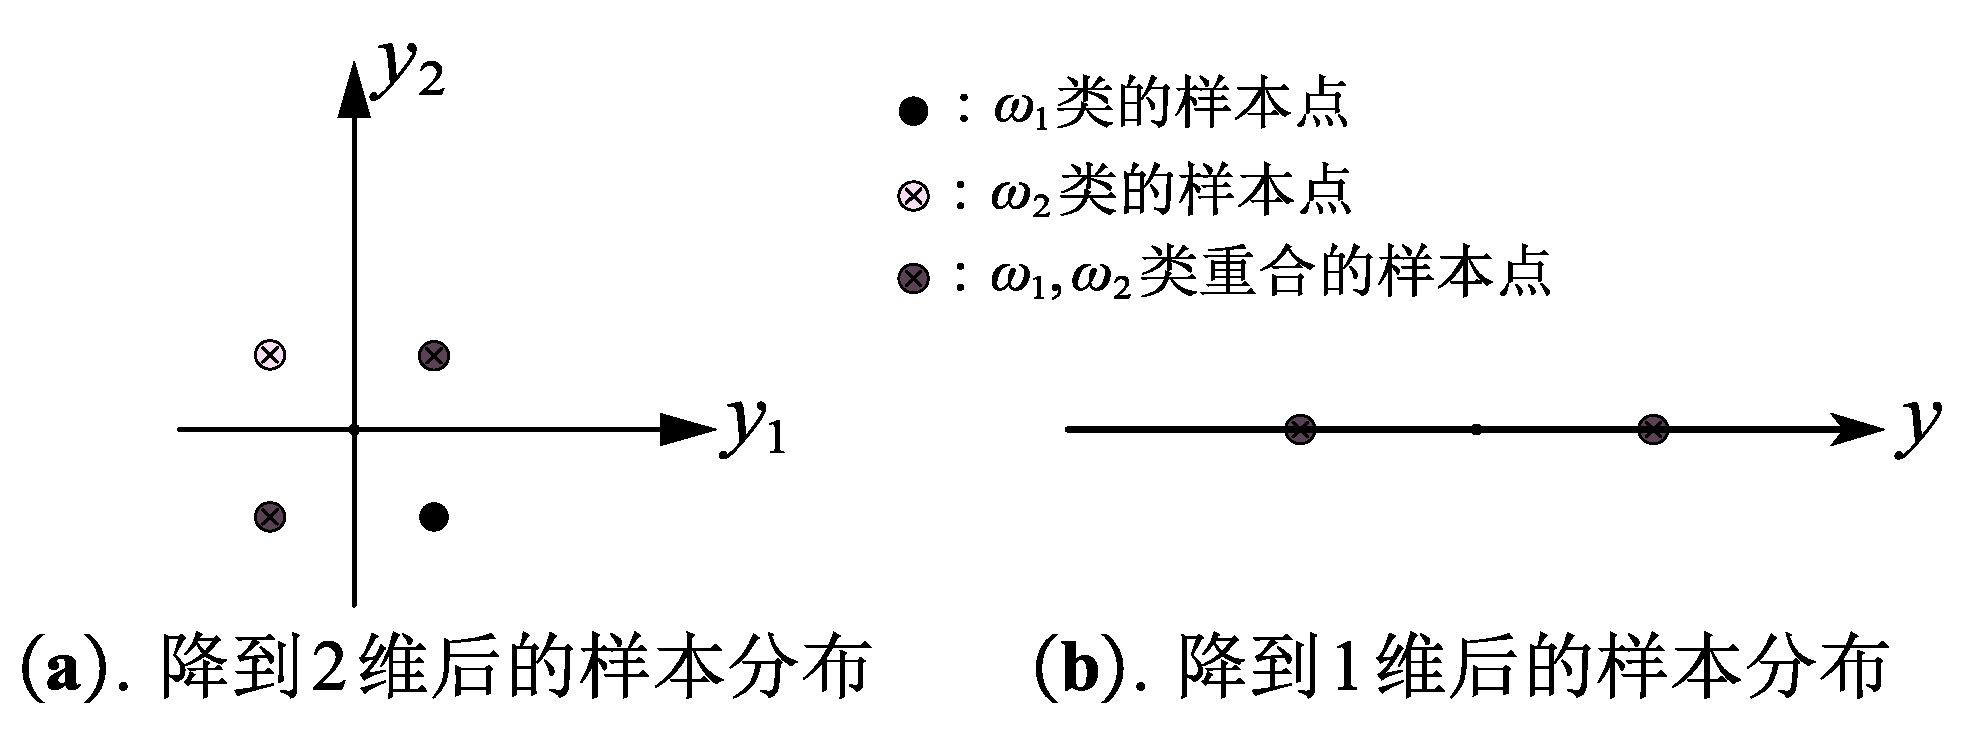
\includegraphics[width=0.6\textwidth]{images/title/样本在降维空间中的位置.pdf}
		\caption{样本在降维空间中的位置}
		\label{fig:样本在降维空间中的位置}
	\end{figure}
	至此, Chap 4 的作业解答完毕.

	\vspace{3cm}

	\begin{figure}[H]  % 这里记得用[H]
		\centering
		
\includegraphics[width=0.6\linewidth]{images/title/ucas_logo 1.pdf}
		%\caption{ucas-logo}
		\label{fig:ucas-logo}
	\end{figure}
\end{homeworkProblem}

% 引用文献
%\bibliographystyle{unsrt}  % unsrt:根据引用顺序编号
%\bibliography{refs}


\end{document}
